\input{head.inc}

% Präambelbefehle für die Präsentation
\title[TET: Elektrostatik-I]{Elektrostatik-I}

\begin{document}
% 
% Frontmatter 
% 
%%%%%%%%%%%%%%%%%%%%%%%%%%%%%%%%%%%%%%%%%%%%%%%%%%%%%%%%%%%%%%%%%%%%%%%%%%%%%%%%%%%%%%%%%%%%%%%%%%%%%%%%%%%%%%%%%%%%%%%%%%%%% 

%% inserts the title page and the table of contents
\maketitle

% 
% Content 
% 
%%%%%%%%%%%%%%%%%%%%%%%%%%%%%%%%%%%%%%%%%%%%%%%%%%%%%%%%%%%%%%%%%%%%%%%%%%%%%%%%%%%%%%%%%%%%%%%%%%%%%%%%%%%%%%%%%%%%%%%%%%%%% 
\section{Elektrostatik}

\begin{frame}
  \frametitle{Elektrostatik: Vakuum und leitenden Körpern}

    %\begin{column}{.3\textwidth}
		\centering
		\resizebox{.9\linewidth}{!}{%
                  \begin{tikzpicture}[line width = 1.2pt, line join=round,x=1.5cm,y=1.5cm,z={(-0.35355cm,-0.35355cm)},>=stealth]
	% Koordinatensystem
	\draw [->] (-0.5,0) -- (5,0) node[anchor=west] {$x$};
	\draw [->] (0,-0.5) -- (0,3) node[anchor=south] {$y$};
	\draw [->] (0,0,-1) -- (0,0,2) node[anchor=north east] {$z$};
	% Differenzvektor R
	\draw [->, color=red!60] (1,1.8) -- (4.5,2.5);
	\draw [color=red!60] (3.8,2.25) node[anchor=south east] {$\ortsvektor[v] = \ortsvektor[v] - \ortsvektor[vs] $};
	% Aufpunkt
	\draw [->,color=blue!70] (0,0) -- (4.5,2.5) node[anchor=west] {$\punkt$};
	\filldraw [color=blue!70] (4.5,2.5) circle (2pt);
	% Ladungsdichte
	\coordinate (a) at (2.1,1.8);
	\coordinate (b) at (2,1.2);
	\coordinate (c) at (1.8,0.4);
	\coordinate (d) at (1.3,0.6);
	\coordinate (e) at (0.7,0.5);
	\coordinate (f) at (0.5,2);
	\coordinate (g) at (1.2,2.5);
	\shade[ball color=white!10!green!20,opacity=0.20] plot [smooth cycle, tension = 1] coordinates {(a) (b) (c) (d) (e) (f) (g)};
	\draw [color=darkgreen] plot [smooth cycle, tension = 1] coordinates {(a) (b) (c) (d) (e) (f) (g)} node [sloped, above] {\ $ \laddichte{V} $};
	\draw [->,color=darkgreen] (0,0) -- (1,1.8);
	\draw [color=darkgreen] (0.5,1.0) node[anchor=north east] {$ \ortsvektor[vs] $};
\end{tikzpicture}}
    %          \end{column}
     %         \end{columns}

  %\begin{coulmns}
    %\begin{column}{0.7\textwidth}
\end{frame}
   \begin{frame}
  \frametitle{Elektrostatik: Vakuum und leitenden Körpern}

                \begin{block}{Problem}
    Im Lösungsgebiet gibt als Quelle eine Ladungsverteilung
    $\rho_v(\ortsvektor[v])$. Abgesehen davon ist der Raum entweder Vakuum
    mit $\varepsilon=\varepsilon_0$ oder kann als perfekt leitend
    $\kappa \to\infty$ angesehen
    werden.

    \alert{Statik:} Die Relaxation der freien Ladungsträger in den perfekt
    leitenden Gebieten ist so schnell, dass alle elektrischen Felder
    praktisch instantan kompensiert werden:
    $$
    \efeld[v] = \vec{0} \text{ in den perfekt leitenden Gebieten}
    $$

    \alert{gesucht:} Feld im Raum außerhalb der perfekten Leiter
  \end{block}
  \begin{block}{Nebenbemerkung}
    \alert{später, bei harmonischer Anregung:} komplexe
    Dielektrizitätskonstante
    $$
    \underline{\varepsilon}(\omega) = \varepsilon'+j\varepsilon'' =\varepsilon(\omega) - j \frac{\kappa(\omega)}{\varepsilon_0\omega}
    $$
    \end{block}
  %\end{column}

  \end{frame}
\begin{frame}
    \onslide<+->{\begin{block}{Grundgleichungen (außerhalb der perf. leitenden Gebiete)}
    \begin{align*}
	& \rotation \efeld[v] = \vec{0}
		&& \oint\limits_{\rand(\flaeche)} \efeld[v] \cdot \intweg[v] = 0\\
	& \divergenz \verschiebung[v] = \divergenz \left( \varepsilon_0 \cdot \efeld[v] \right) = \laddichte{V}
		&& \only<-1|handout:0>{\varepsilon_0\oiint\limits_{\oberfl(\volumen)}
                   \efeld[v] \cdot \intflaeche[v] =
                   \iiint\limits_{\volumen} \laddichte{V} \intvolumen
                   = \ladung \text{ in V}}
                   \only<2->{\boxed{\varepsilon_0\oiint\limits_{\oberfl(\volumen)}
                   \efeld[v] \cdot \intflaeche[v] =
                   \iiint\limits_{\volumen} \laddichte{V} \intvolumen
                   = \ladung \text{ in V}}}
\end{align*}

\end{block}}
\onslide<+->{
In einfachen Fällen (geeignete Symmetrie) kann aus dem obigen
\alert{Colomb-Gauss-Integral} direkt das E-Feld berechnet werden.
}

  
\end{frame}

\begin{frame}
  \begin{exampleblock}{Kugelsymmetrische Ladungsverteilung am
      Ursprung}
    $$
    \rho_V (\ortsvektor[vs]) =  \rho_v(r') \qquad \efeld[v] (\ortsvektor[vs]) = E(r')\einheitsvek{r'}
    $$
    V: Kugel mit Radius r um den Ursprung: $\intflaeche[v] =
    \intflaeche \einheitsvek{r'}  \rightarrow \alert{\efeld[v] \cdot
      \intflaeche[v] = \efeld(r) \intflaeche}$

    \begin{align*}
    \oiint\limits_{\oberfl(\volumen)}
                   \efeld[v] \cdot \intflaeche[v] = & \efeld(r) \oiint\limits_{\oberfl(\volumen)}
                                                       \intflaeche = 4\pi r^2 \efeld(r) \\
      = & \frac{1}{\varepsilon_0} \iiint\limits_{\volumen}
           \laddichte{V} \intvolumen =  \frac{1}{\varepsilon_0} \int_0^r \rho_v(r') r'^2\upd r'
           \int_0^{2\pi} \upd \varphi \int_0^\pi \sin\vartheta
          \upd\vartheta \\
      = & \frac{4\pi}{\varepsilon_0}\int_0^r \rho_v(r') r'^2\upd r'\\
       \efeld(r) = & \frac{1}{\varepsilon_0 r^2} \int_0^r \rho_v(r') r'^2\upd r'
    \end{align*}
    Homogen geladene Kugel mit Radius R; keine Ladung außerhalb:
   $$
    \rho_V (\ortsvektor[vs]) = \begin{cases}
      \rho_V  & \text{ für } r' \le R\\
      0 & \text{ für } r' > R
    \end{cases};\quad \efeld(r) =  \begin{cases}
      \frac{\rho_V}{\varepsilon_0r^2}\frac{1}{3}r^3 =
      \frac{\rho_V}{3\varepsilon_0}r= \frac{Q r}{4\pi\varepsilon_0 R^3}& \text{ für } r \le R\\
      \frac{\rho_V}{\varepsilon_0r^2}\frac{1}{3}R^3 = \frac{Q}{4\pi\varepsilon_0r^2} & \text{ für } r > R
    \end{cases}
    $$
 
    
    \end{exampleblock}
  \end{frame}

  \begin{frame}
    \frametitle{Coulomb-Gauss-Integral: Vorteile - Nachteile}
    \begin{itemize}[<+->]
      \item Die Berechnung des E-Feldes aus dem
        \alert{Coulomb-Gauss-Integral}
        $$
        \oiint\limits_{\oberfl(\volumen)}
                   \efeld[v] \cdot \intflaeche[v] = \frac{1}{\varepsilon_0}
                   \iiint\limits_{\volumen} \laddichte{V} \intvolumen
                   $$
      ist ein guter und intuitiver Lösungsweg, wenn das \alert{linke Integral}
      leicht zu einem Ausdruck für $\efeld[v](\ortsvektor[v])$ für alle
      $\ortsvektor[v]$ im Lösungsvolumen umgeformt werden kann.
      \item Ob das \alert{rechte Integral} dann \alert{analytisch}
        gelöst werden kann, ist grundsätzlich sekundär.
        \item Eine
        analytische Lösung ist zwar in jedem Fall vorzuziehen, aber im
        Zweifel kann as Integral immer \alert{numerisch} gelöst
        werden.
        \item Leider kann das \alert{linke Integral} jedoch nur
          ausgewertet werden, wenn \alert{starke Symmetrien} vorliegen
          (wie im gezeigten Beispiel).
        \item Weitere Beispiele:
          \begin{itemize}
          \item geladener Ring
          \item unendlich langer, homogen geladener Zylinder
          \end{itemize}
          \item Wir benötigen \alert{allgemeinere Methoden} und
              \alert{Methoden für weitere Spezialfälle}!
      \end{itemize}
    \end{frame}

    \begin{frame}
      \frametitle{Coulomb-Integral - Skalarpotential}
      \begin{itemize}[<+->]
        \item Für die \alert{Überlagerung} (Superposition) von $n$
          einzelnen Punktladungen $q_j$ an Positionen $\ortsvektor[v]_j$ ist
          das Feld bekannt, falls keine weiteren
          \alert{Randbedingungen im Endlichen} vorliegen:
          $$
          \efeld[v] (\ortsvektor[v])= \frac{1}{4\pi\varepsilon_0} \sum_{j=1}^n \frac{q_j\left(\ortsvektor[v]-\ortsvektor[v]_j\right)}{\left|\ortsvektor[v]-\ortsvektor[v]_j\right|^3}
          $$
          \item Beim Übergang auf eine \alert{kontinuierliche
              Ladungsverteilung}
            $$
            \upd q =
            \laddichte{V}(\ortsvektor[vs])\upd^3r'$$

            ergibt sich sofort das \alert{Coulomb-Integral}

            $$
          \efeld[v] (\ortsvektor[v])= \frac{1}{4\pi\varepsilon_0}
          \int
          \frac{\laddichte{V}(\ortsvektor[vs])\left(\ortsvektor[v]-\ortsvektor[vs]\right)}{\left|\ortsvektor[v]-\ortsvektor[vs]\right|^3
          } \upd^3r'
          $$
        \item Es gilt
          $$
          \frac{\ortsvektor[v]-\ortsvektor[vs]}{\left|\ortsvektor[v]-\ortsvektor[vs]\right|^3}
            = -\gradient_r \frac{1}{\left|\ortsvektor[v]-\ortsvektor[vs]\right|}
            $$
          \item und somit
            $$
            \efeld[v](\ortsvektor[v]) = -\gradient \phi \quad\text{mit}\quad
            \boxed{\phi(\ortsvektor[v]) = \frac{1}{4\pi\varepsilon_0}
          \int
          \frac{\laddichte{V}(\ortsvektor[vs])}{\left|\ortsvektor[v]-\ortsvektor[vs]\right|} \upd^3r'} \quad\alert{\text{Skalarpotential}}
            $$
        \end{itemize}
      \end{frame}
    
    \begin{frame}
      \frametitle{Skalarpotential formal - Poisson/Laplace-Gleichungen}
      
      \onslide<+->{\begin{block}{Lemma von Poincar{\'e}}
        \begin{itemize}[<+->]
        \item Ein auf einem einfach-zusammenhängenden Gebiet definiertes
        \alert{wirbelfreies Vektorfeld} kann als \alert{Gradient eines
          Potentialfeldes} dargestellt werden.
        $$
        \rotation \vec{\alpha} = \vec{0} \Rightarrow \vec{\alpha} = \gradient f
        $$
        \item Ein \alert{quellenfreies Vektorfeld} auf einem konvexen
        Gebiet kann durch \alert{Rotation eines Vektorpotentials} dargestellt
        werden.
        $$
        \divergenz \vec{\beta} = 0 \Rightarrow \vec{\beta} = \rotation \vec{\alpha}
        $$
      \item Eine \alert{skalare
        Felddichte} kann als \alert{Divergenz eines
        Vektorfeldes} dargestellt werden können.
      $$
      \gamma \text{ ist ein Volumen-Integrand} \Rightarrow \gamma = \divergenz\vec{\beta}
      $$
        \end{itemize}
      \end{block}}
    \onslide<+->{E-Feld: $\boxed{\rotation \vec{E} = \vec{0} \Rightarrow \vec{E}
      = -\gradient\phi}$; \enquote{-}: Konvention; $\phi$:
  \alert{Elektrisches Skalarpotential}}
      \end{frame}
    
      \begin{frame}

        \begin{itemize}[<+->]
        \item Für statische Probleme gilt immer \qquad$\rotation\vec{E} = \vec{0}$
        \item daher: \hspace{4cm} $\vec{E} = - \gradient \phi$
          \item Für \alert{einfache} Medien mit $\verschiebung[v] = \varepsilon \efeld[v]$:\qquad $\divergenz \vec{E} =
            \frac{1}{\varepsilon} \laddichte{V} $
          \item einsetzen:
            \begin{align*}
            \divergenz \vec{E} = &
                             \frac{1}{\varepsilon} \laddichte{V}\\
              \divergenz\left(-\gradient \phi\right) =& \frac{1}{\varepsilon}
                                              \laddichte{V}\\
            \Aboxed{\laplace \phi = & - \frac{1}{\varepsilon}
                                      \laddichte{V}} & \text{\alert{
                                                       Poisson-Gleichung}}\\
              \text{Spezialfall } \laddichte{V}=0 \to\quad \Aboxed{\laplace \phi = & 0} & \text{\alert{
                                                       Laplace-Gleichung}}
            \end{align*}
            \item Vorteil: Ist $\phi$ die Lösung des Problems, erfüllt
              das zugehörige $\vec{E} = - \gradient \phi$ \alert{automatisch} die
              zweite Gleichung $\rotation\vec{E} = \vec{0}$
              \item Nachteil: Anstelle von zwei DGLs erster Ordnung nun
                eine \alert{DGL zweiter Ordnung}.
                \item Bemerkung: $\efeld[v](\phi + \text{const.}) =
                  \efeld[v](\phi)$, $\phi$ nur bis auf additive
                  Konstante bestimmt.
          \end{itemize}

        
        \end{frame}

\begin{frame}
\frametitle{Kraft - Feldlinie - Äquipotentialfläche}

\begin{itemize}[<+->]
\item Kraft auf eine Probeladung $q$ im Feld $\efeld[v](\ortsvektor[v])$
$$
\vec{F}(\ortsvektor[v]) = q \efeld[v](\ortsvektor[v])
$$ 
\item Die \alert{Trajektorie} einer solchen fiktiven Testladung
  beschreibt eine \alert{Feldlinie} (Orientierung: von \enquote{+}
  nach \enquote{-}). 
\item Orte mit gleichem Skalarpotential $\to$
  \alert{Äquipotentialfläche}
\item Sei $\upd\vec{s}$ eine kleine Verschiebung auf einer
  Äquipotentialfläche, dann gilt:
\begin{align*}
\upd \phi = & \phi(\ortsvektor[v]+\upd\vec{s}) - \phi(\ortsvektor[v]) \equiv 0\\
 = & \gradient \phi \cdot \upd\vec{s}
\end{align*}
also:
$$
\gradient \phi \perp \upd\vec{s} \land \gradient \phi \parallel \efeld[v] \to
\boxed{\efeld[v] (Feldlinien) \perp \text{Äquipotentialflächen}}  
$$
\end{itemize}

\end{frame}

\begin{frame}
\frametitle{Wegunabhängigkeit - Potentialdifferenz}
\begin{columns}[T]
\begin{column}{.4\linewidth}
  \resizebox{.8\columnwidth}{!}{%
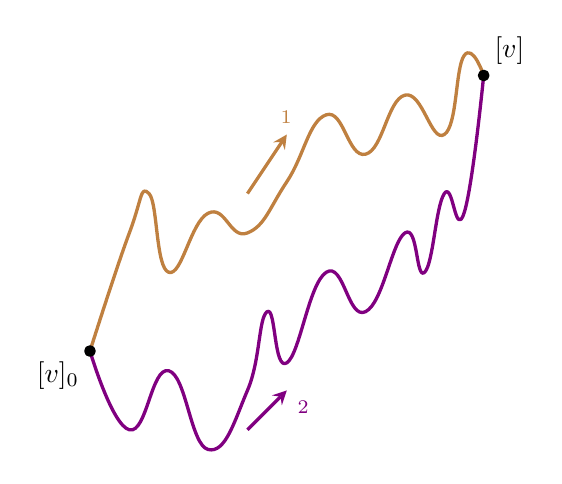
\begin{tikzpicture}[line width = 1.2pt, line join=round,x=0.5cm,y=0.5cm,>=stealth]
	% Koordinaten der Punkte
	\coordinate (a) at (0,0);
	\coordinate (b) at (10,7);
	% Weg 1
	\draw [color=brown] plot[smooth,tension=0.8] coordinates{(a) (1,3) (1.5,4) (2,2) (3,3.5) (4,3) (5,4.3) (6,6) (7,5) (8,6.5) (9,5.5) (9.5,7.5) (b)};
	\draw[->,color=brown] (4,4) -- (5,5.5) node[anchor=south] {$\rand_1$};
	% Weg 2
	\draw [color=violet] plot[smooth, tension=0.8] coordinates{(a) (1,-2) (2,-0.5) (3,-2.5) (4,-1) (4.5,1) (5,-0.3) (6,2) (7,1) (8,3) (8.5,2) (9,4) (9.5,3.5) (b)};
	\draw[->,color=violet] (4,-2) -- (5,-1) node[anchor=north west] {$\rand_2$};
	% Punkt 0
	\filldraw (a) circle (1.5pt);
	\draw (a) node[anchor=north east] {$\ortsvektor[v]_0$};
	% allgemeiner Punkt
	\filldraw (b) circle (1.5pt);
	\draw (b) node [anchor = south west] {$\ortsvektor[v]$};
\end{tikzpicture}}
\resizebox{1.1\columnwidth}{!}{%
\begin{tikzpicture}[line width = 1.2pt,
  line join=round,
  scale=1,
  x=0.5cm,
  y=0.5cm,
  >=stealth]
	% Koordinaten der Punkte des Weges
	\coordinate (a) at (0,2);
	\coordinate (b) at (8,5);
	\coordinate (c) at (2,3);
        \coordinate (d) at (-2,4.3); 
        \coordinate (e) at (9.6,2.5);

	% Rechte Winkel
	\draw (0.6,2.4) arc (10:120:0.4cm);
	\filldraw (0.05,2.6) circle (1pt);
	\draw (7.7,5.8) arc (120:210:0.4cm);
	\filldraw (7.62,5.2) circle (1pt);
	% Fläche 1
	\draw plot[smooth, tension = 0.8] coordinates{(-3,5) (a) (0,-2)}; 
	\draw [decorate, decoration={markings,
    mark=between positions 0.2 and 0.5 step 3mm with
    {\arrow[green]{latex}}}] plot[smooth, tension = 0.8] coordinates{(-3,5) (a) (0,-2)}; 
	\draw (0,-2) node[anchor=north] {$\elpotential(\ortsvektor[v]_0)$};
	% Fläche 2 
	\draw  plot[smooth, tension = 0.8] coordinates{(7,8) (b) (e) (10,2)}; 
	\draw  [decorate, decoration={markings,
    mark=between positions 0.6 and 0.95 step 3mm with
    {\arrow[green]{latex}}}] plot[smooth, tension = 0.8] coordinates{(7,8) (b) (e) (10,2)}; 
	\draw (10,2) node[anchor=north west] {$\elpotential(\ortsvektor[v])$};
	% Punkte
	\draw (a) circle (1.5pt);
	\draw (a) node[anchor=north east] {$\ortsvektor[v]_1$}; 
	\draw (b) circle (1.5pt);
	\draw (b) node[anchor=south west] {$\ortsvektor[v]_2$}; 
	\draw (d) circle (1.5pt); 
	\draw (d) node[anchor=south west] {$\ortsvektor[v]_0$}; 
	%\draw [color=green] plot[smooth] coordinates{(d) (f) (a)}; 

	\draw (e) node[anchor=north east] {$\ortsvektor[v]$};
        \draw (e) circle (1.5pt); 

	% Weg
	\draw [color=magenta] plot[smooth, tension=0.8] coordinates{(a) (c) (6,4) (b)}; 
	\draw [decorate, , decoration={markings,
    mark=between positions 0.1 and 0.99 step 3mm with
    {\arrow[green]{latex}}}] plot[smooth, tension=0.8] coordinates{(a) (c) (6,4) (b)}; 
	\draw [->,color=magenta] (c) -- ++(3,{2/5*3}) node[anchor=south] {$\efeld[v]$};
	\draw [->,color=blue] (c) -- ++(2,{2/5*2}) node[anchor=south east] {$\upd \weg[v]$};
\end{tikzpicture}}
\end{column}
\begin{column}{.6\linewidth}
  \begin{itemize}[<+->]
    \item Betrachte zwei beliebige Wege $C_1$ und $C_2$ zwischen
      $\ortsvektor[v]_0$ und $\ortsvektor[v]$.
      \item Wegen $\rotation \efeld[v] =\vec{0} $ gilt für jeden geschlossenen
        Weg $C$:
        $
        \oint_C \efeld[v]\cdot\upd\vec{s} = 0 
        $
        \item Der Weg $C_1 + (-C_2)$ ist ein geschlossener Weg. Daher
          folgt die \alert{Wegunabhängigkeit}:
          $$
       \boxed{\int_{\ortsvektor[v]_0, C_1}^{\ortsvektor[v]} \efeld[v]\cdot\upd\vec{s} =        \int_{\ortsvektor[v]_0, C_2}^{\ortsvektor[v]} \efeld[v]\cdot\upd\vec{s}} 
       $$
       \item Wege auf Äquipotentialfläche ($\ortsvektor[v]_0\to\ortsvektor[v]_1$ und
         $\ortsvektor[v]_2\to\ortsvektor[v]$) tragen nicht bei, da $\upd\vec{s}
         \perp \efeld[v]$
         \item Wege entlang einer Feldlinie ($\ortsvektor[v]_1\to\ortsvektor[v]_2$):
           $\efeld[v]\cdot\upd\vec{s} = E \upd s = -|\gradient\phi| \upd s$
         \item Somit
           $$
             \boxed{\int_{\ortsvektor[v]_0}^{\ortsvektor[v]} \efeld[v]\cdot\upd\vec{s} = 
                                                                       -
                                                                       \int_{\ortsvektor[v]_1}^{\ortsvektor[v]_2}
                                                                       |\gradient\phi|\upd
                                                                       s
                                                                       =
                                                                       \phi(\ortsvektor[v]_0)
                                                                       - \phi(\ortsvektor[v])}
             $$
    \end{itemize}
\end{column}
\end{columns}
\end{frame}

\begin{frame}
  \frametitle{Spannung und Arbeit}
  \begin{block}{Spannung}
    Man definiert die
    \alert{Spannung} $U_{21}$ als \alert{Potentialdifferenz}:
    $$
    U_{21} = \phi_2 - \phi_1 = - \int_{\ortsvektor[v]_1}^{\ortsvektor[v]_2}
    \efeld[v]\cdot \upd \vec{s}; \quad [U] = \si{\volt}
    $$
    \end{block}
    \begin{block}{Arbeit}
      Auf eine Probeladung $q$ wirkt im E-Feld die elektrostatische
      Kraft $\vec{F}_e = q\efeld[v]$. Um die Ladung am Ort
      festzuhalten ist eine gegengerichtete Kraft aufzuwenden
      $\vec{F}_\text{mech} = -\vec{F}_e$. Die \alert{Arbeit} $A$
      auf dem Weg von $\ortsvektor[v]_1$ nach $\vec{r_2}$ ist somit
      $$
      A = \int_{\ortsvektor[v]_1}^{\ortsvektor[v]_2}
      \vec{F}_\text{mech}\cdot\upd\vec{s} = - \int_{\ortsvektor[v]_1}^{\ortsvektor[v]_2}
      \vec{F}_e\cdot\upd\vec{s} = -q\int_{\ortsvektor[v]_1}^{\ortsvektor[v]_2}
      \efeld[v]\cdot\upd\vec{s} = q (\phi(\ortsvektor[v]_2)-\phi({\ortsvektor[v]_1)})
      = q U_{21}  
      $$
     
    \end{block}
\end{frame}

% \begin{frame}
%   \frametitle{Energie und Energiedichte}
%     \begin{block}{Energie}
%       Arbeit = Änderung der potentiellen Energie. Damit ist \alert{die
%         elektrostatische Energie}
%       $$
%       \boxed{W_e(\ortsvektor[v])= q \phi(\ortsvektor[v])} \quad [W_e] =
%       \si{\volt\ampere\second} = \si{\watt\second} 
%       $$
%       Durch Vergleich mit der elektrostatischen Kraft findet man
%       $
%       W_e = -\vec{F}_e\cdot\upd \vec{s} \Rightarrow \boxed{\vec{F}_e =
%       -\gradient W_e = q\efeld[v]}$
%       \end{block}
%     \begin{block}{Energiedichte}
%       Durch den Übergang $q\to\laddichte{V}$ ergibt sich aus der
%       Energie die \alert{elektrostatische Energiedichte}
%       $$
%       \boxed{w_e(\ortsvektor[v])= \laddichte{V}(\ortsvektor[v]) \phi(\ortsvektor[v])} \quad [w_e]  = \si{\watt\second\per\meter\cubed} 
%       $$
%       Wie oben ergibt sich eine \alert{elektrostatische Kraftdichte}
%       $
%       \boxed{\vec{f}_e =
%       -\gradient w_e = \laddichte{V}\efeld[v]} $
%       \end{block}

%     \end{frame}

\begin{frame}
  \frametitle{Elektrostatische Energie}
  \begin{block}{Definition}
    Die \alert{Energie} einer auf einen \alert{endlichen Raum} beschränkten
    Ladungskonfiguration $\laddichte{V}$ entspricht der Arbeit, um
    Ladungen aus dem Unendlichen zu dieser Konfiguration zu bringen.

    Wegen $\phi(\ortsvektor[v]) =
    \frac{1}{4\pi\varepsilon_0}\int\frac{\laddichte{V}(\ortsvektor[vs])}{\left|\ortsvektor[v]-\ortsvektor[vs]\right|}
    \upd^3r$ ist \alert{$\phi(\infty) = 0$} für eine räumlich begrenzte Ladungsverteilung.
  \end{block}
  \begin{itemize}[<+->]
  \item $N$ Punktladungen: Potential am Ort $\ortsvektor[v]_i$ der ersten $(i-1)$ Punktladungen
    mit Ladung $q_j$ an den Orten $\ortsvektor[v]_j$:
    $$
    \phi(\ortsvektor[v]_i) = \frac{1}{4\pi\varepsilon_0} \sum_{j=1}^{i-1}
    \frac{q_j}{|\ortsvektor[v]_i - \ortsvektor[v]_j|}
    $$
    Arbeit um Ladung $q_i$ von $\infty$ nach $\ortsvektor[v]_i$ zu bewegen: $A_i = q_i\phi(\ortsvektor[v]_i)$

    Die Gesamtarbeit $A = \sum_{i=2}^N A_i$ (der Term für $i=1$
    verschwindet, da der Raum bei der Verlagerung der ersten Ladung
    noch feldfrei ist) entspricht der \alert{elektrostatischen
      Energie} $W_e$:
    $$A = W_e = \frac{1}{4\pi\varepsilon_0} \sum_{i=2}^N \sum_{j=1}^{i-1}
    \frac{q_i q_j}{|\ortsvektor[v]_i - \ortsvektor[v]_j|} = \frac{1}{\alert{8}\pi\varepsilon_0} \sum_{i=1}^N \sum_{j=1}^{N}
    \frac{q_i q_j}{|\ortsvektor[v]_i - \ortsvektor[v]_j|} \alert{(1-\delta_{ij})}
    $$
    \end{itemize}
  \end{frame}
  \begin{frame}
    \frametitle{Elektrostatische Energie - kontinuierliche Verteilung}
    \begin{itemize}[<+->]
      \item In der Formel für $N$ Punktladungen tauchen die Terme
        $i=j$ nicht auf.
        \item Beim Übergang auf kontinuierliche Ladungsverteilungen
          lassen sie sich aber nicht ausschließen. Der \alert{nicht
            völlig Äquivalente} Ausdruck heißt in diesem Fall somit:
          $$
         \boxed{ W_e = \frac{1}{8\pi\varepsilon_0} \iint
    \frac{\laddichte{V}(\ortsvektor[v]) \laddichte{V}(\ortsvektor[vs])}{|\ortsvektor[v]-
      \ortsvektor[vs]|} \upd^3 r\upd^3 r' = \frac{1}{2} \int
    \laddichte{V}(\ortsvektor[v])\phi(\ortsvektor[v]) \upd^3 r}
  $$
  \item Nebenbemerkung: Die Diskussion des Unterschieds führt zum Begriff der
    \alert{Selbstenergie} einer Punktladung, der jedoch (bisher) nicht
    widerspruchsfrei aufgeklärt werden kann. Das ist nicht völlig
    überraschend, da Punktladungen nur Modelle sind.
    \item Mit $\laddichte{V}=-\varepsilon_0\laplace\phi$ und
      $\divergenz(\phi\gradient\phi) = \gradient\phi\gradient\phi + \phi\laplace\phi$
      folgt
      \begin{align*}
      W_e = & -\frac{\varepsilon_0}{2}\left(\int \divergenz(\phi\gradient\phi)
      \upd^3 r - \int (\gradient\phi)^2 \upd^3 r\right)  =
                     \frac{\varepsilon_0}{2} \int (\gradient\phi)^2 \upd^3 r\\
        = & \frac{\varepsilon_0}{2} \int |\efeld[v]|^2 \upd^3 r
            \quad\alert{Energiedichte:} \boxed{w_e = \frac{\varepsilon_0}{2} |\efeld[v]|^2}
      \end{align*}
    \end{itemize}
    \end{frame}

    \input{finalframe.inc}
   
\end{document}